%!TEX root = jt-thesis-main.tex

\section{English Abstract}
\begin{onehalfspace}
	
	The english abstract is required for all english theses at TU-Berlin.
\end{onehalfspace}
\clearpage

\section{Deutscher Abstract}
\begin{onehalfspace}
	
	Ein deutscher Abstract wird immer benötigt, für alle Abschlussarbeiten an
	der TU-Berlin. 
\end{onehalfspace}
\clearpage


\section{Introduction}
\label{sec:Introduction}
Gartner Inc. states that the number of interconnected devices will reach 20.4
billion by 2020 \footnote{Gartner Inc., R. (2017, February 7). Gartner Says 8.4
Billion Connected "Things" Will Be in Use in 2017, Up 31 Percent From
2016.Retrieved September 28, 2018, from
https://www.gartner.com/en/newsroom/press-releases/2017-02-07-gartner-says-8-billion-connected-things-will-be-in-use-in-2017-up-31-percent-from-2016}.
To gather information from those devices, we need algorithms which efficiently
sample and route data from sensor nodes (i.e., devices) to data sinks. Energy
expenditure will gain higher importance, especially for mobile devices such as
battery-powered wearables and smartphones. A \ac{WSN} is often battery-powered
and use cases span from home and health applications to the military
sector~\cite{akyildiz2002wireless}. With low production costs of a node as a
goal in \acp{WSN}~\cite{akyildiz2002wireless}, resource usage at the nodes is
restricted. While reducing sampling frequencies leads to a higher life of a
battery-powered sensor network, important changes in the observed phenomenon
could be missed which reduces the quality of the
data~\cite{akyildiz2002wireless}. A tradeoff between the quality of data and
energy expenditure arises, thus an optimization is needed. 
\par
Different methods for optimizing \acp{WSN} were presented in surveys
(e.g.,~\cite{abbasi2007survey},~\cite{sivrikaya2004time},~\cite{carrano2014survey}).
The proposed areas of optimization include clustering
algorithms~\cite{abbasi2007survey}, time
synchronization~\cite{sivrikaya2004time}, duty
cycling~\cite{carrano2014survey}, topology control~\cite{li2013survey},
in-network aggregation~\cite{fasolo2007network}, data
compression~\cite{srisooksai2012practical}, and general routing
techniques~\cite{al2004routing}~\cite{kulkarni2011particle}~\cite{singh2015survey}~\cite{rault2014energy}.
TinyDB~\cite{madden2005tinydb}, ACQUIRE~\cite{sadagopan2003acquire} and
COUGAR~\cite{yao2002cougar} introduce system architectures for query processing
which consist of algorithms for sampling, and routing data requested by a user
through a SQL-like language.


\subsection{Motivation}
\label{sec:motivation}

As stated above, surveys and taxonomies were presented for different areas of
sensor networks. However, during our research, we did not encounter a survey or
catalog focusing on sampling algorithms in sensor networks. This thesis aims to
provide a catalog for a comprehensive overview of the existing sampling
algorithms for the specific use case of sensor data. For researchers as well as
practitioners, a collection of sampling algorithms is a valuable starting point
for finding a solution for a design problem in a sensor network. 
\par
Thus, a taxonomy of the algorithms will be presented to provide a compact
overview. Furthermore, algorithms which focus on areas other than sensing (like
routing and topology building) in sensor networks will be presented.
Combinations of said algorithms with sampling algorithms as well as
combinations of sampling algorithms from different categories could inspire
further research.


\subsection{Scientific Background}
\label{sec:Scientific Background}

Different types of \acp{SN}, like \acp{WSN}, \acp{RSN}, or wired \acp{SN}
exist. While all of them are used to monitor a phenomenon, like the temperature
in a room \footnote{Madden, S. et al. 2004. Intel Lab Data. [ONLINE] Available
at: http://db.csail.mit.edu/labdata/labdata.html. [Accessed 29 November 2018].}
or the behaviour of wildlife~\cite{bennett2011cranetracker} performance
indicators vary in their significance. Intuitively, wired \acp{SN} do not
consider energy expenditure as the primary concern. \acp{RSN} have a way to
collect energy from the environment they are stationed at, through, e.g. solar
and wind or more exotic variants like vibration \footnote{Perpetuum. 2018.
Technology. [ONLINE] Available at: https://perpetuum.com/technology/. [Accessed
29 November 2018].}. To enable perpetual data collection in \acp{RSN},
techniques for allocating sensing tasks to sensors while handling the non
linear emission of, e.g. solar and wind is crucial~\cite{liu2011perpetual}.
\acp{WSN} often have a limited energy source at their disposal, making
management of energy expenditure a top priority to increase network lifetime.
As Cheng et al. state in their work~\cite{cheng2013stcdg} network lifetime is
often defined in \acp{WSN} as the lifetime of the first node to run out of
energy. 
\par
\acp{WSN} and \acp{RSN} are often designed with some nodes sensing the
phenomenon and one or more sink nodes wich transfer the sensed data to a
central base station. Based on the type of topology, e.g. a simple star
structure\ref{fig:topologies}, sensed data is forwarded to the sink node
directly, i.e. in a one-hop manner. More complex topologies, e.g. tree
\ref{fig:topologies} or connected star structures, often require to relay
sensed data through intermediary nodes to a sink node in a multi-hop fashion,
as direct communication paths between sensing and sink nodes are not always
possible~\cite{romer2004design}. 
\par
In more complex topologies with a lot of intermediary nodes, finding the
optimal routing path from sensor node to the sink is not trivial. With
increasing number of nodes, the complexity of the computation of the optimal
route increases, as nodes have multiple neighbors from which to choose the next
transmission step. Solving such a problem locally, i.e. nodes compute the next
best step, with additional contraints, e.g. minimizing energy expenditure and
meet quality of data thresholds can be an unfeasible task. On the other hand,
outsourcing this task to the basestation could induce a major communication
overhead with additional energy expenditure. Techniques on topology building
and route path finding will be discussed later in the thesis.

\begin{figure}%
    \centering
    \subfloat[Star
    Topology]{{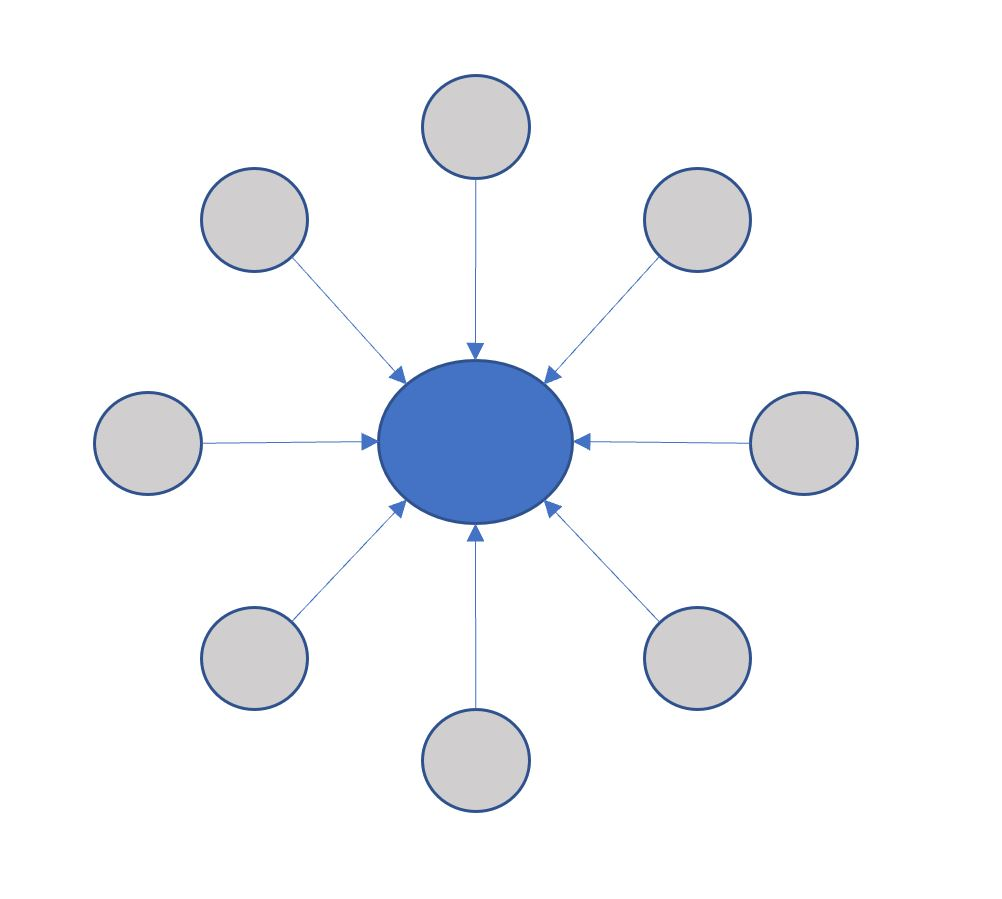
\includegraphics[width=5cm]{images/topology-star-no-legend.jpg}
    }}%
    \qquad
    \subfloat[Tree
    Topology]{{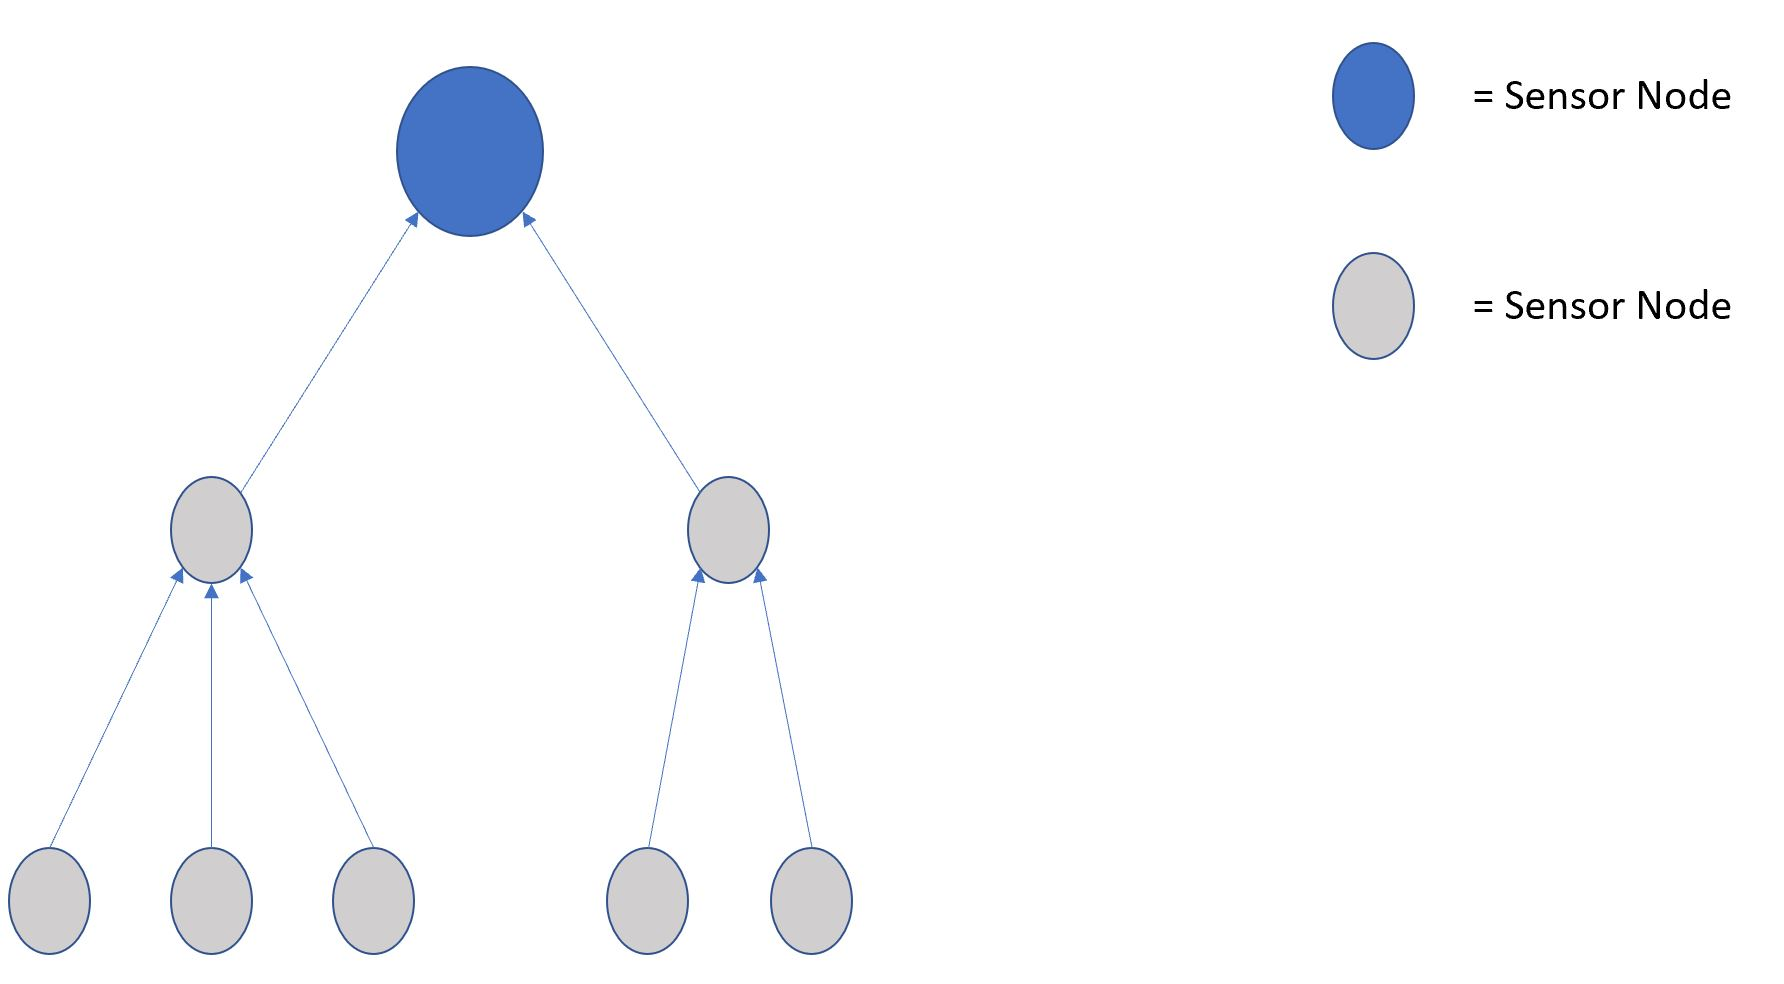
\includegraphics[width=5cm]{images/topology-tree.jpg} }}%
    \caption{Example Topologies. Inspiration taken from Reina et
    al.~\cite{reina2013role}}% \label{fig:topologies}%
\end{figure}


\FloatBarrier


\subsection{Contributions}
\label{sec:contributions}

The contributions of this thesis go as follows: 
\begin{enumerate}
	\item A catalog of different sampling algorithms for sensor data gathering
	\item A taxonomy of those algorithms for a compact overview of the field of data sensing in \acp{SN}
	\item Combinations of different algorithms to provide a basis for further
	research
\end{enumerate}


\subsection{Thesis Outline}

\para{Section \ref{sec:Taxonomy}.}  In section \ref{sec:Taxonomy}, we present a
high level taxonomy for classifying sampling algorithms. The section is split
into four subsections. The first gives an overview of the described classes and
subclasses and a motivation of why we chose such a partitioning. Each following
section describes a class and its subclasses in detail. For each subclass,
relevant information of multiple algorithms will be presented. We define
relevant information as:
\begin{itemize}
	\item The problem(s) the algorithm tries to solve
	\item Basic workings of the algorithm
	\item Experimental results of the algorithm and how it compares to others
	\item Use case(s) (if any)
	\item Advantages and limitations of the algorithm the authors discuss
	\item Compatibility of the algorithms with other techniques
\end{itemize}   


\para{Section \ref{sec:Discussion}.} In section \ref{sec:Discussion}, we review
algorithms not covered in the taxonomy from areas other than sampling, e.g.
topology building and routing. This section is split into two subsections. The
first subsection presents those algorithms and their relevant information. The
definiton of relevant information for those algorithms does not change. In the
second section we discuss possible combinations of different sampling
algorithms with other sampling and non-sampling algorithms. The combinations
found here could be used as a basis for further research.


\section{Taxonomy}
\label{sec:Taxonomy}

In this section we present our taxonomy of sampling algorithms for \acp{SN}. We
classify algorithms into three categories: \catI (Section~\ref{sec:catI}), \catII (Section~\ref{sec:catII})  and \catIII (Section~\ref{sec:catIII}).
%COMMENT JT: Make sure to stay with present tense. We devided=>we devide. (I rephrased the sentence above)

%COMMENT JT: Extend this header such that all subsection are referenced (Manage the expectation of your reader)

%COMMENT JT: I miss some description for each of these categories. I would appreciate if yu extend the paragraph above with one sentence for each cateforey. e.g., "Sampling Algorithms are all algorithms which .... In contrast, filtering algorithms ... Data sharing algorithms apply orthorgonal optimizations ...."

\subsection{Terminology}

%COMMENT JT: I like the idea of this section. However, it doesn't really fit my expectation of a "Taxonomy" section. I added a subsection for terminology definitions. This is just a suggestion. You should integrate  

The literature related to data retrieval from sensors defines many different terms such as data collection, data sampling, data gathering, and data sensing.
%COMMENT JT: Each of the items in the list above should have at least one reference following it. Better three references.
Some publications use these terms as synonyms while other publications use different terms to differentiate concepts.
In the following paragraphs, we clarify the definitions of data collection, data sampling, data gathering, and data sensing.
%COMMENT JT: I rephrased this paragraph. Please check if you like it.

%COMMENT JT: Make sure to clarify the motivation: Why is the content which follows important? Because we need to clarify the terminology in order to be precise in the following sections...

%COMMENT JT: You may want to use a description environment to highlight the term you are defining in each of the following paragraphs.

%Many different terms for the concept of data retrieval from sensors exist in
%the literature. Data collection, data sampling, data gathering, and data
%sensing could be seen as synonyms, however, we found they are sometimes used in
%different contexts.
\par
Data collection is often mentioned in connection with the whole process of
acquiring data through sensors in \acp{SN}.
% consider this: a query for temperature in a room is pushed down the network.
% a sensor in that room would power up and produce a stream of data... or the
% sensor node gets the instruction to produce data with the sensor e.g. every 3
% sec for 18 sec so sensing would only apply to the process of getting digital
% data via a sensor while sampling could mean the same in context of sampling
% the "real values" of a happend event. Sampling could also mean getting a
% subset of data from multiple sensors.
A data stream produced by a sensor sensing a phenomenon is sampled by an
sampling algorithm. The data is then routed through the network to the
destination. The work of Yao et al.~\cite{yao2015edal} contributes, i.a., a
technique, for finding the lowest cost path for sent data packages in a
\acp{WSN} while additionally employing compressive sampling. The authors use
data collection to define this process. Additionally, a survey by Di Francesco
et al.~\cite{di2011data} defines the term data collection as the process of
getting data from a sensor node to the sink node.
% COMMENT JT: Instead of saying "could be used" you can just say that we use it as such and other do this as well: Similar to related literature, we use the terms A and B as syn. [1,2,3]. In general, each of the definition paragraphs should end with an concluding sentence which clarifies how you use the term you defined.
% COMMENT JT: NEVER write "could be" in research. This basically means you have no idea! In German: "Es könnte sein" => Ja was? Ist es so oder nicht? Kann es sein oder nicht?. Either it can or it cannot. The only place where you could write "could" is in the "future research" section. There you indeed make guesses.
\par
Data gathering on the other hand could be used as a synonym for data
collection. Vukobratovic et al.~\cite{vukobratovic2010rateless} describe data
gathering as the process of collecting sensed data from sensor nodes at
specific sink nodes. A sink node could be a basestation, e.g. a wired server,
or another node in the \ac{SN} which acts as a cluster head. Other works which
use the term data gathering in the same context are often found in the domain
of compressive sensing~\cite{cheng2013stcdg,luo2009compressive,wang2012data}.
%COMMENT JT: Why? Does it have a special meaning to them? (Remember that the paragraph needs a concluding sentence)
%(e.g.~\cite{cheng2013stcdg},~\cite{luo2009compressive},~\cite{wang2012data})
\par
% cite BBQ, they argue that sensing is basically sampling. A sensor net
% monitoring an environment, cannot reflect reality 1:1, but only a fraction of
% it at descreet points in time.
The definitons for data sampling and data sensing are also unclear in the
literature.
%The statement above is very strong. You basically say that noone defined data sampling properly. Better say that the definitions are inconsistent. This is less offensive.
Zhao et al.~\cite{zhao2016cats} employ sampling in the context of
sink nodes assigning sampling tasks, which consist of a time window and a
sampling interval, to sensor nodes. Trihinas et al.~\cite{trihinas2015adam}
also do not differentiate between sampling and sensing. Aquino et
al.~\cite{aquino2014musa} on the other hand, discern sensing as the process of
a preconfigured sensor unit measuring a physical phenomenon and sampling as the
software taking samples form the data generated by the sensor unit. The
distinction is important as the authors point out, that generally, an online
reconfiguration of the sensor sensing times is not possible. Contrary, software
is more flexible and sampling rates and intervals can be specified online.
%COMMENT JT: There's is often a confision between sampling (i.e. reading) from sensors and computing smaller samples (example data) from a huge badge of data (i.e. reservoir sampling). It would be good to clarify the difference here and to point out that we are NOT dealing with the latter one in this thesis.
\par
We will use data collection and data gathering as synonyms and differentiate
between data sensing and data sampling.
%I would make the below part a separate paragraph because above this comment you talk about algorithms  (i.e. software) and below  this comment you, out of a sudden, talk about devices, servers (i.e. hardware).
Additional synonyms are base station,
fusion center and client station which all describe a wired station like a
server to which information is routed and from which user queries can be
specified to then be distributed in the network.
% Sampling Cats - Zhao = sampling interval and sampling tasks a sampling task
%     is alocated to a sensor node by a sink node sampling task has a time
%     window and a sampling interval Adam - Trihinas = adaptive sampling
%     techniques and sampling rate sampling == sensing data with sensors Musa -
%     Aquio = a distinction is made between sampling and sensing sensing =
%     device (sensor) is configured to take regular samples over time sampling
%     = software takes samples from data produced by sensor software is more
%     flexible while sensor sensing generally cannot be reconfigured online

\subsection{Overview}
\label{sec:Overview}
% Picture of taxonomy at the beginning Explain picture and explain the terms
% e.g. model based adaptive sampling is a prediction scheme ... Reasoning
% behind the partitioning of the algorithms maybe if a assignment of a
% particular algorithm is not straightforward
% explain why thesis title is about sampling algorithms and taxonomy has 
% filtering and sampling as different categories


\subsection{\catI} % Sampling Algorithms
\label{sec:catI}

The first category of our taxonomy incorporates all algorithms which primary 
focus is on manipulating the sampling or sensing rate of one or multiple sensor
nodes to reduce data throughoutput. 
 % TODO find papers to cite which, e.g., use sampling and filtering
 % COMMENT JT: "throughput" usually has a psitive annotation. It feels weired that someone what's to reduce "throughput". Maybe replace it by saying sth. like "reduce network utilization", "reduce sensor load"...
Although there are algorithms from other categories which also may incorporate
manipulations to the sensing/sampling rates of sensor nodes, we include
algorithms to the Sampling Algorithms category only if the main focus of the
work lies on sampling.
% COMMENT JT: It would be good to have concrete examples here.

% COMMENT JT: Please add some outlook/summary for the following subsections.

\subsubsection{Adaptive Sampling}
\label{sec:Adaptive Sampling}

% All required definitions for adaptive sampling
Trihinas et al.~\cite{trihinas2015adam} define adaptive sampling as:

\begin{quote}
    "The process of dynamically adjusting the sampling rate to the current
    metric evolution, such that when stable phases in a metric stream are detected,
    the sampling rate is reduced to ease processing and energy consumption."
\end{quote}

%COMMENT JT: I recommend to start a new line after each sentence in the source file. This makes it easier to find a sentence from the PDF in the sources.

\par
% maybe remove backcasting from taxonomy
Although the quote is from 2015, the idea of adaptive sampling goes back to the
2000s. One technique called Backcasting was presented by Willet et
al.~\cite{willett2004backcasting}. The key idea of the work is that a monitored
environment exhibits correlations in time and space domains which can be
exploited to reduce the number of required sensor nodes to deliver an accurate
picture about the monitored environment. The authors assume that the sensor
network is a rectangular field of uniformly distributed sensor nodes.
Initially, a subset of the sensor nodes is chosen by the fusion center to
provide an initial estimate of the sensed phenomenon by a recursive dyadic
partition. A subset of nodes are mutliple clusters of nodes with a cluster head
each. Cluster heads route the data from the sensor nodes to the fusion center
and vice versa. The fusion center recieves the sensed data and activates
additional nodes to improve the quality of the sampling by reducing the
\ac{MSE}. The authors evaluate their approach theoretically and come to the
conlusion, that a \ac{WSN} with 10000 sensors and energy to operate
continuously for a year, would operate for 10 years when using Backcasting. The
authors point out that network lifetime could be improved if mechanisms for
cycling the position of cluster head would be implemented. Altough the
algorithm does not manipulate the sampling rates of individual sensor nodes it
is still one of the first algorithms to adaptively change the sensing tasks of
nodes based on the dynamics of the observed phenomenon.
\par
Another technique, also from 2004, was published by Jain et
al.~\cite{jain2004adaptive}. The authors main contribution is an algorithm to
change the sampling rate of individual sensor nodes in a stream sensor network
based on the importance of the observed data. An important event could be a
camera observing non-standard driving behaviour of a car, e.g. driving in a
zigzag course or a temperature spike in a data center. Locally, kalman filters
predict sensed values. They are then compared against the actual sensed values.
The values are stored in a sliding window locally. An estimation error is
computed over the sliding window. The estimation error indicates a changing
dynamic of a observed phenomenon. After each taken sample, a sensor node
adjusts its \ac{SI} i.e. the time interval between two consecutive samples. If
the desired \ac{SI} lies in the \ac{SIR}, the sensor node can adjust its
\ac{SI} locally. Otherwise the sensor node has to request a new \ac{SI} from
the server. The server keeps a metric of avaliable communication resources
which gets updated after a request to change a \ac{SI} is accepted. The
requests are stored in a job queue. To approve a \ac{SI} a linear optimization
problem has to be solved. The authors evaluated their approach on synthetic
data generated by a spatio-temporal data generator. Tested metrics where the
mean fractional estimation error $ \eta $, the proportion of messages exchanged
between the source and the server and the number of values sensed by the source
nodes \textit{m}. The adaptive sampling algorithm outperformed the alternative
uniform sampling algorithm almost in every test. Tests were done, i.a using
different numbers of sensor nodes and sliding window sizes. The authors
indicate, that the algorithm is not applicabble to multi-hop sensor network,
i.e. a sensor node has to have a direct connection to the server. Furthermore,
both the sliding window and the \ac{SIR} have to be chosen by the user. Also,
the authors state that the message overhead is high. The main goal of the
algorithm is to optimize bandwidth usage in the network, thus this technique is
more suitable for wired \acp{SN} and less for \acp{WSN} as the communication
overhead is high and communication consumes a major amount of energy in
most sensor nodes~\cite{raghunathan2002energy}.
\par
A techinque designed initially for a glacier monitoring application by Padhi et
al. \ac{USAC}~\cite{padhy2006utility} is an example of an adaptive sampling
scheme for a \ac{WSN}. The algorithm uses a linear regression model at each
sensor node to capture phase shifts of the observed phenomenon as fast as
possible. The model predicts values at a sensor node. Those values are checked
against the actual sensed values. If a predicted value lies in the user defined
\ac{CI}, then the sensor node reduces its sampling rate by a multiplicative
factor $ \alpha $ until the sampling rate reaches $ f_{min} $. $ f_{min} $ is
set by the user. If the value does not lie in the \ac{CI} then the sensor node
raises its sampling rate to $ f_{max} $ to capture a supposed change in the
dynamic of the observed phenomenon. The experiments tested the algorithm
against the older deployed protocoll in the glacier monitoring application
\textit{GLACSWEB}. The tests were conducted in a simulated environment using
historical data from the application. The authors tested different network
topologies, numbers of sensor nodes in a network and number of changes in the
dynamic of the data. The experiments resulted in \ac{USAC} outperforming the
older algorithm in every test. The efficiency increase, which is defined by the
authors as

\begin{quotation}
    "The value of the data gained over the energy consumed) of USAC relative to
    GLACSWEB in each case."
\end{quotation}

was, i.a. 470\% when distributing sensor nodes randomly around a center base station.
\par

Lorem Ipsum 
\subsubsection{Compressive Sampling}
\label{sec:Compressive Sampling}


\subsection{\catII}
\label{sec:catII}

\subsubsection{Model Based Schemes}
\label{sec:Model Based Schemes}


\subsubsection{Adaptive Filtering}
\label{sec:Adaptive Filtering}

\subsection{\catIII}
\label{sec:catIII}


\section{Discussion}
\label{sec:Discussion}


\subsection{Other Algorithms}
\label{sec:Listings}

\subsubsection{Routing}
\label{sec:Listings}

\subsubsection{Topology Building}
\label{sec:Listings}


\subsection{Combination of Algorithms}
\label{sec:Listings}


\section{Conclusion}
\label{sec:Conclusion}


\section{References}
\label{sec:References}

